\section{Introduction}
\subsection{Qu'est-ce qu'un système multiphysique ?}

Pour comprendre le fonctionnement des systèmes qui nous entourent, il est souvent nécessaire de maîtriser un voire plusieurs domaines de la physique. En effet, le winch utilisé dans le laboratoire a un fonctionnement essentiellement mécanique. En revanche, le simulateur de drone $D^2C$ est composé d'une partie mécanique (rotation du banc et des hélices) une partie électrotechnique (moteurs) une partie électronique (commande des moteurs) une partie informatique (gestion de la commande et des informations). 

Pour modéliser un système, plusieurs outils peuvent être nécessaires. Lorsqu'un outil est associé à un champ de la physique, on peut parler de modèle << mono physique >> :
\begin{itemize}
\item pour modéliser la géométrie d'un système ou le comportement d'un mécanisme, on peut faire appel à SolidWorks par exemple;
\item pour modéliser la partie électrique d'un système il est possible d'utiliser un logiciel comme PSpice;
\item pour programmer une interface graphique d'un logiciel, il est possible d'utiliser Python...
\end{itemize}

En revanche, lorsqu'on veut que tous ces domaines communiquent, il faut une plate forme commune permettant l'échange entre les modèles. On parle alors de modélisation multiphysique. Il est possible d'utiliser des logiciels comme Scilab (Xcos -- Modelica) ou Matlab (Simulink -- Simscape). 



\subsection{Pourquoi modéliser des systèmes ?}
Dans l'industrie, les modèles sont indispensables. Ils permettent d'avoir un modèle numérique, image du produit que l'on cherche à réaliser ou que l'on a déjà. L'image doit être aussi fidèle à la réalité que possible. On a vu que ce modèle peut-être << monophysique >> ou << multiphysique >>. 

L'objectif du modèle est de se substituer au produit réel. Les simulations réalisées sur le modèle ont pour objectif de remplacer des expérimentations sur le produits, considérées comme coûteuse en temps et en argent. 

Il est possible de recenser les avantages et inconvénients liés à la simulation des modèles \cite{1}. 
%\begin{multicols}{2}
\begin{itemize}[label=\ding{51}]
\item Pouvoir prévoir le comportement du système réel alors qu'il n’existe pas encore lors de la phase de conception;
\item permettre la prévision de phénomènes (en météorologie par exemple);
\item éviter ou limiter le recours aux expérimentations réelles qui peuvent être très
coûteuses ou très dangereuses, voire proscrites (essais nucléaires militaires) ou
impossibles dans l’état actuel des connaissances et des moyens (projet ITER) ;
\item quand l’échelle de temps des phénomènes dans le système réel ne permet pas une
expérience « en une durée raisonnable » pour effectuer des observations ou des mesures.
(premiers instants de l’univers ($t < 10^{-6} \text{s}$) ou l'évolution des galaxies
($t>10^6$ années);
\item « observer » ou représenter des variables inaccessibles à l'expérience ou la mesure;
\item les manipulations sont faciles sur un modèle. Elles peuvent être répétées, voire itérées
automatiquement pour apprécier de très nombreuses situations ;
\item le droit à l’erreur, sans risque ;
\item la possibilité de supprimer des phénomènes perturbateurs ou des effets
secondaires.
\end{itemize}
%\vfill\null
%\columnbreak

\begin{itemize}[label=\ding{56}]
\item Avoir une confiance aveugle dans les simulations et ses résultats : des erreurs liées aux
modèles ou aux calculs peuvent ne pas être perçues immédiatement ;
\item « oublier » les conditions de la simulation et les hypothèses formulées pour établir le
modèle et surtout dans le cas des systèmes complexes ;
\item « inverser » la réalité et « forcer » le réel à intégrer les contraintes du modèle ;
\item oublier le niveau de précision des résultats provenant du modèle.
\end{itemize}
%\end{multicols}


%\newpage

\section{Modélisation des systèmes multiphysiques}[Systèmes multiphysiques]
\subsection{Modélisation causale et acausale}

%\begin{multicols}{2}
Lorsque le fonctionnement d'un système est régit par une équation différentielle, dont l'ordre de dérivation de la sortie est supérieur à l'ordre de dérivation de l'entrée, la sortie est une conséquence de l'entrée. En passant l'équation dans le domaine de Laplace puis en la traduisant sous forme de schéma bloc, on obtient alors un bloc \textbf{orienté} traduisant ainsi la relation de cause à effet entre l'entrée et la sortie. 

On parle ici de modélisation \textbf{causale}. 

Les liens entre les blocs représentent une grandeur physique (courant, tension, position, vitesse \textit{etc}.).

%\vfill\null
%\columnbreak

En modélisation acausale, les entrées et sorties ne sont pas spécifiées. Les liens entre entrées et sorties sont définies de manière implicite. Lorsqu'on visualise la traduction graphique d'un modèle acausal, les liens ne sont pas orientés (les blocs sont << réversibles >>). Les blocs sont traversés par des flux d'énergie d'un même domaine physique.  

Dans Matlab -- Simulink, on parle de grandeurs potentielles (across) et de grandeur traversante (through) : 
\begin{itemize}
\item une variable potentielle est mesurée par un instrument
en parallèle avec la chaîne d’énergie;
\item une variable traversante est mesurée par un instrument
en série avec la chaîne d’énergie.
\end{itemize}

Dans Scilab -- Coselica, (langage Modelica), on parle de variables potentielles et flux.
\begin{itemize}
\item variables potentielles: les variables qui sont reliées au même port sont égales;
\item variables flux : les variables qui aboutissent au
même port ont pour somme 0.
\end{itemize}
%\end{multicols}


\begin{table*}[h!]
\caption{Modélisation acausale dans Matlab -- Simulink -- Simscape : variables << across >> et << through >>.}
\begin{tabular}{lll}
\midrule
Domaine physique & Variables << across >> &  Variables << through >> \\ \hline
Électrique & Tension (\si{V})& Courant (\si{A})\\ 
Hydraulique & Pression (\si{Pa})& Débit (\si{m^3.s^{-1}})\\ 
Mécanique de translation & Vitesse linéaire (\si{m.s^{-1}})& Force (\si{N})\\ 
Mécanique de rotation & Vitesse angulaire(\si{rad.s^{-1}}) & Moment (\si{Nm})\\ 
%Pneumatique & Pression (V)& Débit massique (V)et flux d'entropie \\ \hline 
Thermique & Température (K)& Flux thermique et flux d'entropie \\ 
\bottomrule
\end{tabular}
\end{table*}

\subsection{Les différents modèles et outils}

La figure ci-dessous présente un modèle causal et un modèle acausal du système de laboratoire <<~Control'X~>> en utilisant le logiciel Matlab-Simulink.

\begin{figure*}[!h]
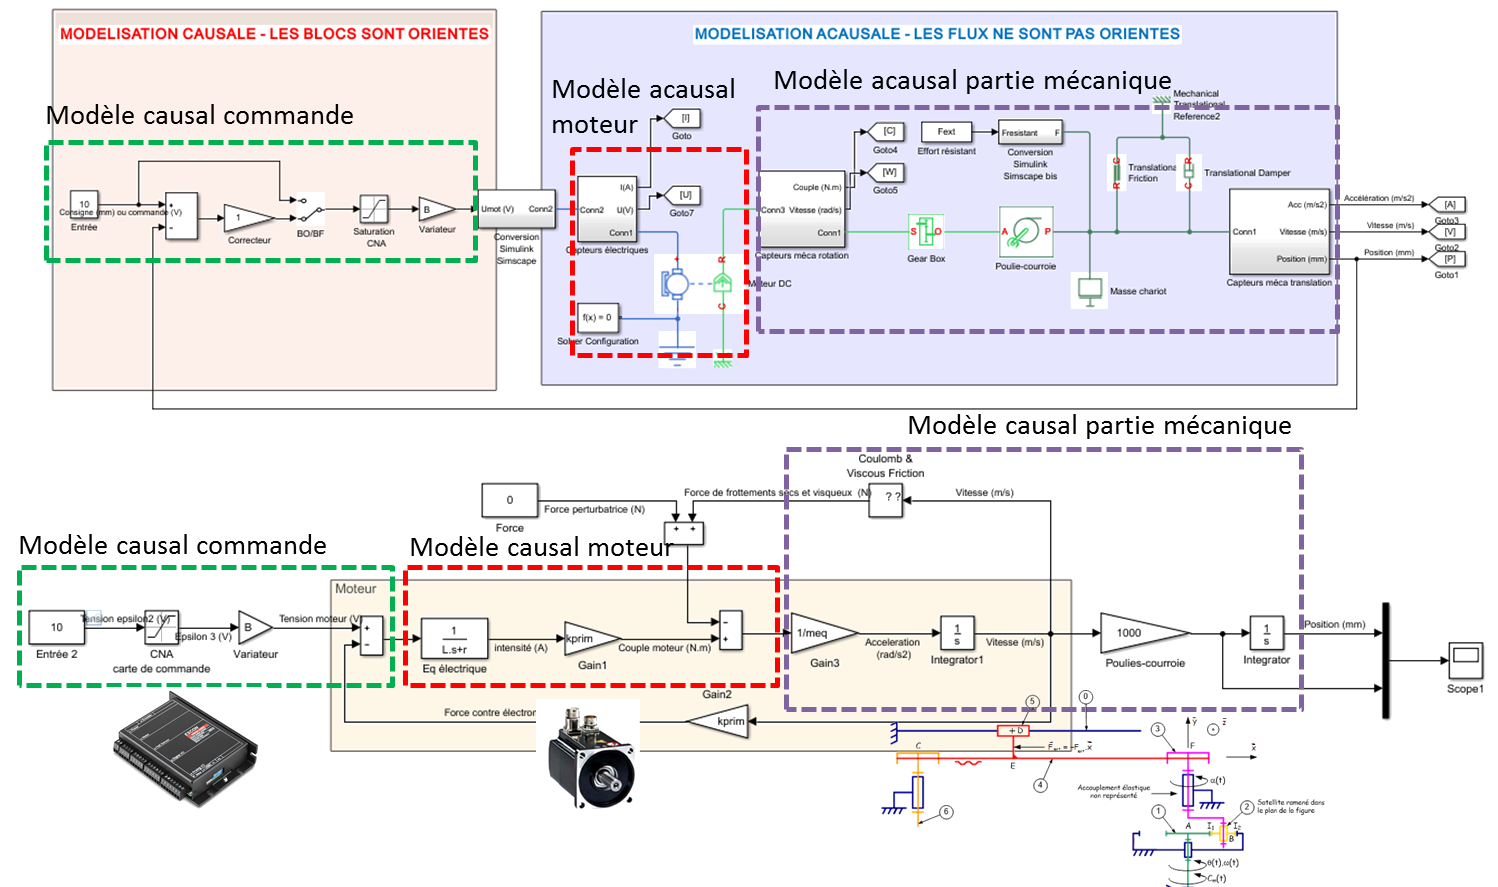
\includegraphics[width=\linewidth]{Modeles}
\end{figure*}

Visuellement on constate que sur le modèle causal, les composants du système apparaissent. Ainsi, sans connaître les lois de comportements des composants, il est possible de réaliser le modèle multiphysique d'un système.

En modélisation acausale, on utilise une représentation par schéma-blocs. Il est ici indispensable de connaître les modèles de connaissance ou de comportement des composants pour réaliser le modèle.

\subsection{Résolution -- Avantage et Inconvénients}

\begin{marginfigure}
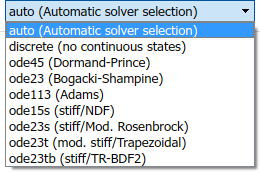
\includegraphics[width=\linewidth]{solveur}
\caption{Solveurs Matlab}
\end{marginfigure}

Que ce soient des modèles causaux ou acausaux, Matlab a recours à des solveurs pour simuler le comportement des systèmes. En effet, des équations différentielles, linéaires ou non, sont << cachées >> derrière les blocs.  

Par défaut, nous laisserons un choix automatique du solveur. Cependant, certains modèles imposeront (via un message d'erreur) le changement de ce solveur. Par ailleurs le pas de simulation devra être changé dans certain cas, dans le but d'améliorer la précision des résultats.




\begin{warn}
Attention, il est à noter qu'il peut être difficile de réaliser de diagramme de Bode en utilisant un modèle acausal. Ceci peut être un handicap en phase de conception d'un système car il devient plus délicat de déterminer les résonances du système.
\end{warn}
\section{Modélisation des systèmes physiques}[Modélisation mono-physique]
On utilisera ici Matlab -- Simulink. Certains modèles sont aussi transposables avec Scilab -- Xcos. 

\subsection{Modélisation des systèmes mécaniques}
\subsubsection{Introduction}

\begin{marginfigure}[-1.5cm]
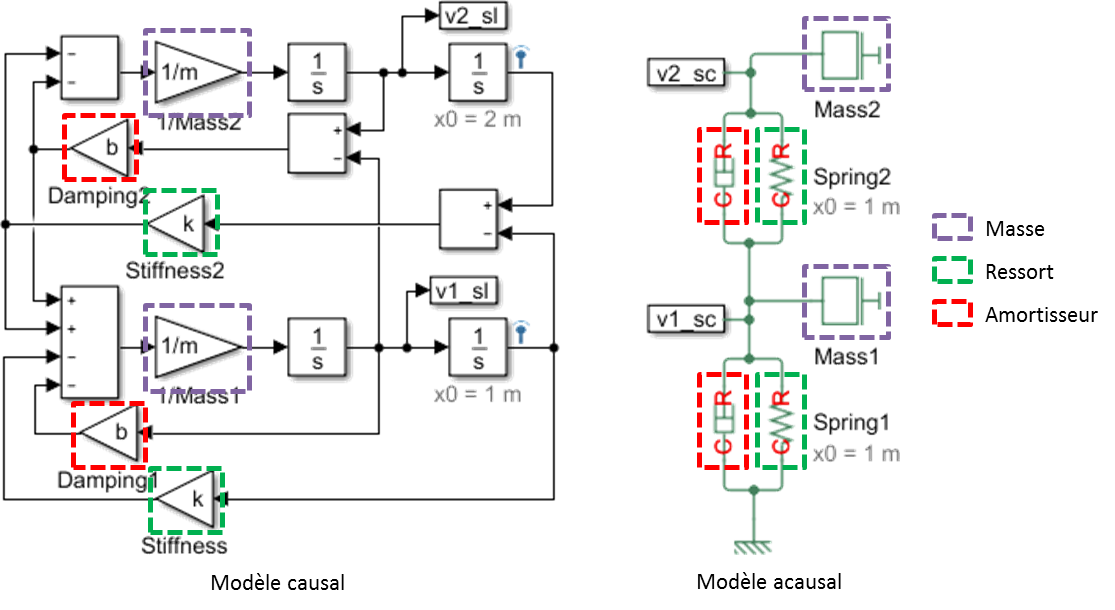
\includegraphics[width=\linewidth]{Masse_Ressort}

\caption{Modélisation causale et acausale d'un système avec deux systèmes << masse -- ressort -- amortisseur >> en série.}
\end{marginfigure}

Deux modes de modélisation des systèmes mécanique est disponible : une modélisation 1D (mouvement de translation suivant une seule direction, mouvement de rotation autour d'un axe fixe) ou une modélisation 3D. 
La modélisation 1D est possible directement dans Matlab. Pour la modélisation 3D, il est plus aisé d'utiliser SolidWorks. 


\begin{figure}[!h]
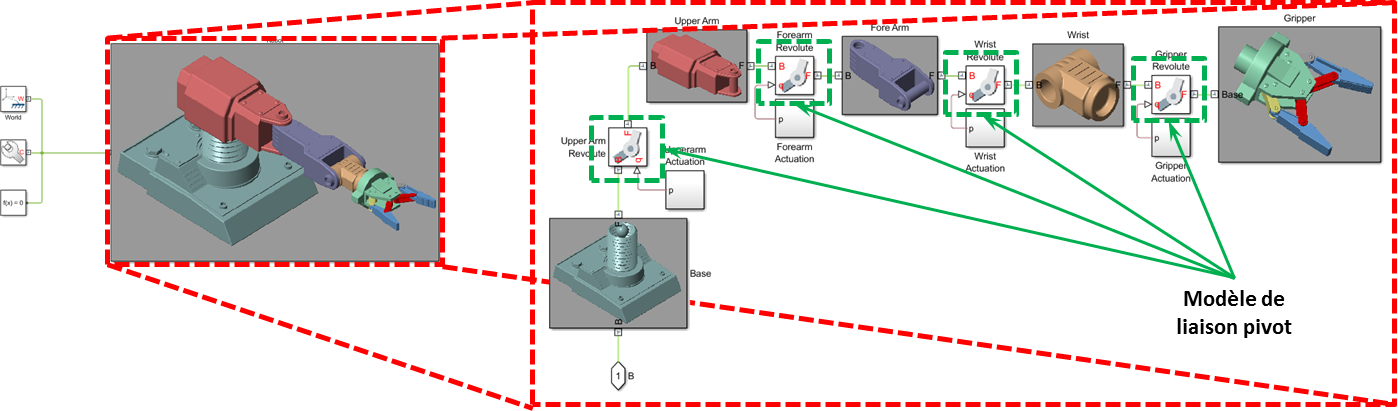
\includegraphics[width=\linewidth]{Modele3D}

\caption{Modélisation acausale 3D d'un bras robotisé.}
\end{figure}

\subsubsection{Blocs communément utilisés en modélisation multiphysique.}
Les éléments communément utilisés sont donnés dans la figure suivante. 

\begin{figure*}[!h]
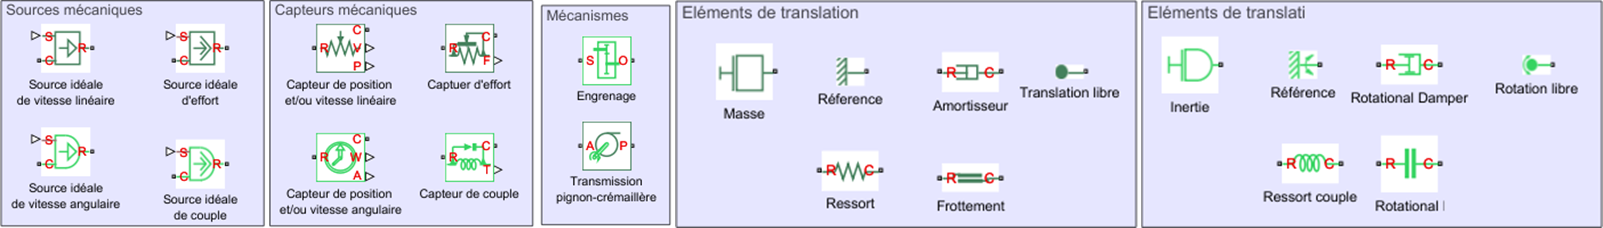
\includegraphics[width=.9\linewidth]{Bilbio_SimMeca_02}
\end{figure*}

La figure suivante illustre une transmission mécanique modélisée en utilisant Simulink. On notera le positionnement des capteurs pour mesurer des variables accross ou through, ainsi que le positionnement du bloc permettant de modéliser les frottements.

\begin{center}
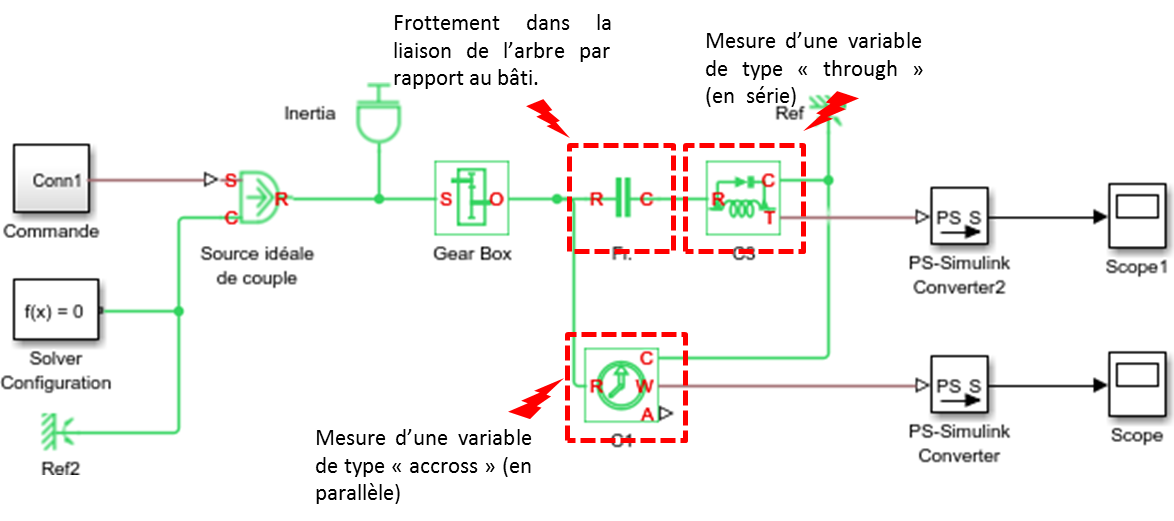
\includegraphics[width=.9\linewidth]{transmission_meca}
\end{center}

\subsection{Modélisation des systèmes électriques}

\begin{figure}[!h]
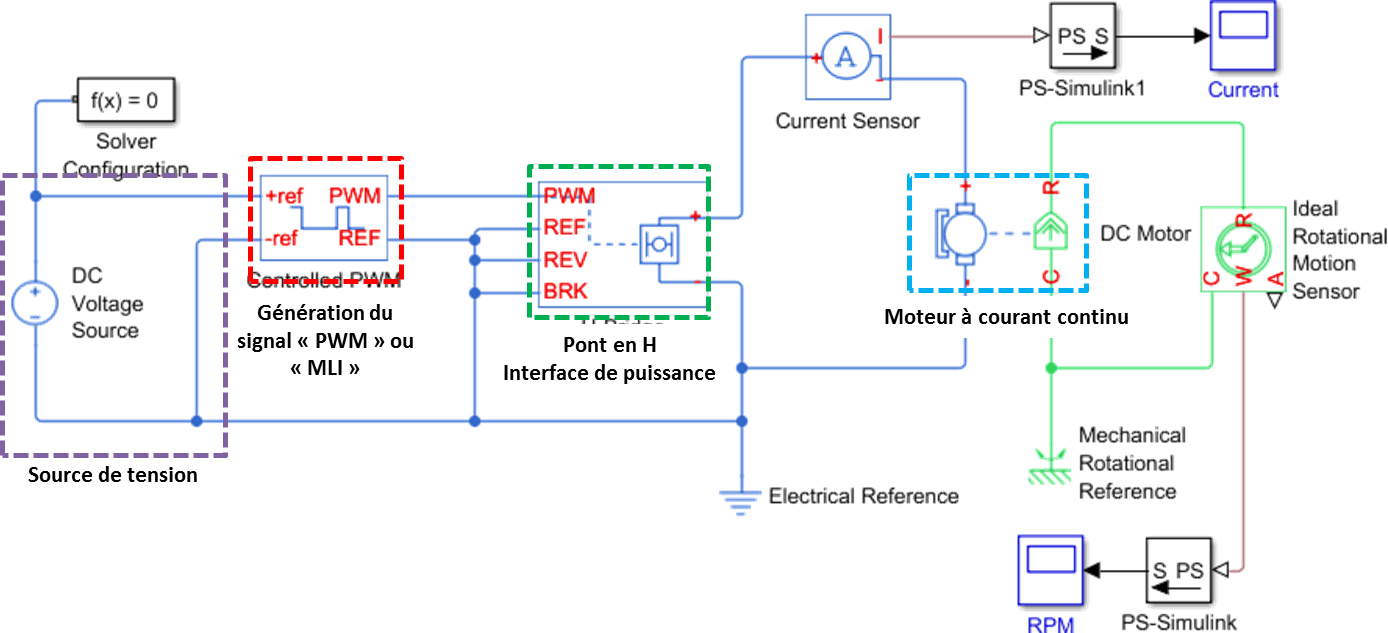
\includegraphics[width=\linewidth]{MoteurCC}

\caption{Modélisation acausale de la commande d'un moteur à courant continu.}
\end{figure}


\subsection{Modélisation des systèmes thermiques, pneumatiques et hydrauliques}
En cas de besoin, des exemples complémentaires sont disponibles en utilisant Maltab -- Simulink.

%\subsection{Modélisation des interfaces}

\section{Modélisation des non-linéarités}[Non-linéarités]

Même si on cherche à modéliser les blocs d'un système par des équations linéaires (à coefficients constants), il est très fréquent de rencontrer des systèmes (notamment mécaniques) qui n'obéissent pas des lois linéaires (par exemple, le comportement du Maxpid est non linéaire : suivant la plage de fonctionnement -- entre 0 et 5\textdegree ou entre 85 et 90\textdegree -- un tour de moteur ne correspond pas au même mouvement angulaire du bras). 

Deux solutions s'offrent alors à nous : linéariser le fonctionnement ou modéliser la non linéarité. 
Les modèles causaux sont par essence linéaire. Cependant, il est possible d'intégrer des non-linéarités modélisables relativement simplement (seuil, saturation, hystérésis). Il est en revanche plus délicat de modéliser les non linéarités géométriques des mécanismes. 
En revanche dans les modèles acausaux, la passerelle entre SolidWorks et Matlab, permet par exemple de modéliser des systèmes mécaniques non linéaires.

\textbf{Attention : l'analyse fréquentielle d'un système non linéaire n'a pas (peu ?) de sens, même s'il est possible d'effectuer un diagramme de Bode, notamment avec Matlab...}

\subsection{Linéarisation}
Lorsqu'un système est non linéaire, il peut être possible de le linéariser. Cela signifie que \textbf{localement} (sur un certain intervalle) on approxime le comportement du système par une droite. On conséquence, on conserve la validité de notre modélisation de type SLCI. Cependant, il faut faire attention à la zone de validité du modèle : si le comportement du système est fortement linéaire la linéarisation ne sera valable que dans une certaine zone.


\begin{marginfigure}[2cm]
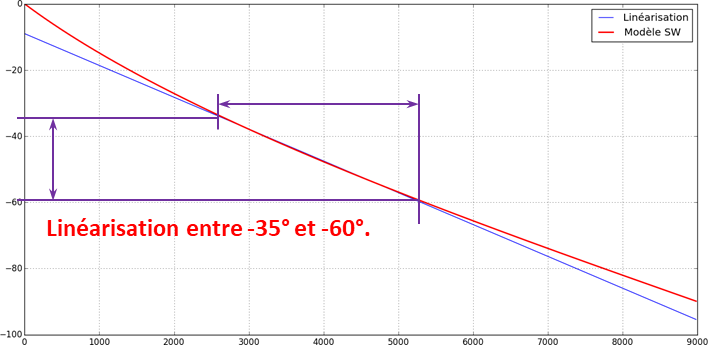
\includegraphics[width=\linewidth]{Maxpid_linearisation_02}
\end{marginfigure}

\begin{exemple}[title=Exemple -- Loi entrée sortie du Maxpid]
%\textit{Loi entrée sortie du Maxpid}
Le comportement mécanique du Maxpid n'est pas linéaire. Si on désire modéliser ce comportement sur un système causal, il est impératif d'utiliser une loi linéaire. 

Dans le premier cas, on modélise le comportement en utilisant une régression linéaire. 
Ce modèle génère des erreurs, mais il est <<~utilisable~>> sur toute la plage de fonctionnement. 

Il est aussi possible, dans un second cas, de linéariser le système autour d'un point de fonctionnement. Ainsi, le modèle sera plus fidèle à la réalité autour de ce point de fonctionnement. Par contre, les écarts s'accroissent en s'éloignant du point de fonctionnement. 

\end{exemple}

\subsection{Saturation}

\begin{marginfigure}
\centering
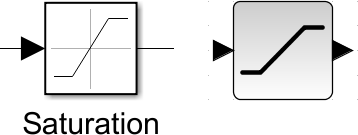
\includegraphics[width=.8\linewidth]{sat}

Paramètres : $s_{\text{max}}$ et $s_{\text{min}}$
\end{marginfigure}

\begin{marginfigure}
\centering
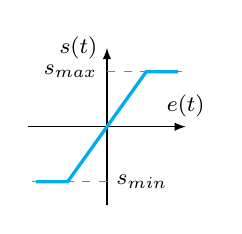
\begin{tikzpicture}
\draw [-latex] (0,-1) -- (0,1) node [left]{\footnotesize $s(t)$};
\draw [-latex] (-1,0) -- (1,0) node [above]{\footnotesize $e(t)$};
\draw [cyan,very thick] (-.9,-.7) -- (-.5,-.7) -- (.5,.7) -- (.9,.7);
\draw [dashed,cyan] (0,.7) node [left,black]{\footnotesize $s_{\text{max}}$}-- (1,.7);
\draw [dashed,cyan] (0,-.7) node [right,black]{\footnotesize $s_{\text{min}}$}-- (-1,-.7);
\end{tikzpicture}
\end{marginfigure}

Même si vous l'avez peut-être peu remarqué, les saturations sont omniprésentes sur les systèmes réels. Les principales sources de saturation sont des saturations en tension ou des saturations en courant. 

En régime saturé, au delà d'une certaine valeur d'entrée, le signal de sortie du bloc reste identique et égal à la valeur de saturation.




Tout d'abord, dans les systèmes asservis et corrigés, le correcteur permet souvent une amplification de la consigne. Par exemple, un correcteur proportionnel de valeur 5 dans la boucle ouverte permet de multiplier par 5 la tension de commande. Celle-ci peut alors être supérieure à la tension que la source peut fournie.

De même, suivant la charge agissant sur un système (charge électrique ou mécanique), le courant nécessaire à un déplacement peut devenir très important, notamment en phase transitoire. Un pic de courant peut avoir pour effet de détériorer des composants.


\begin{marginfigure}
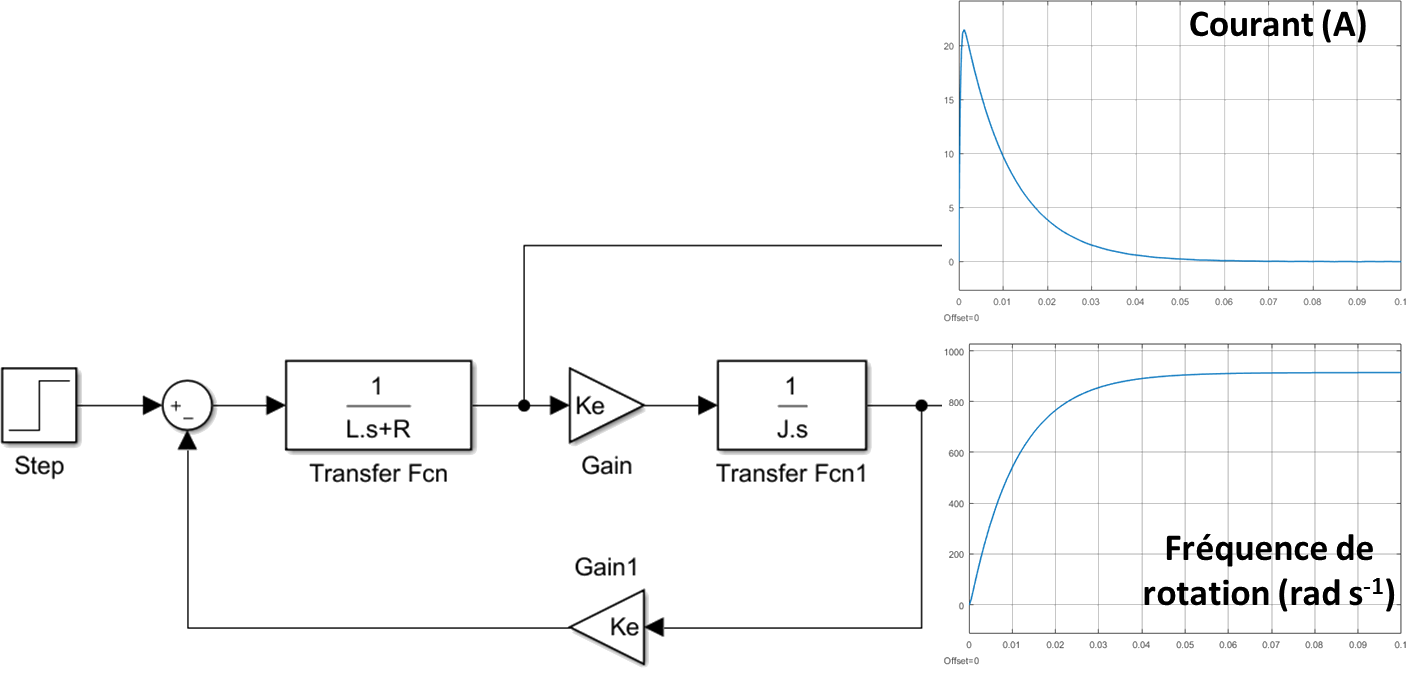
\includegraphics[width=\linewidth]{Modele_MCC}

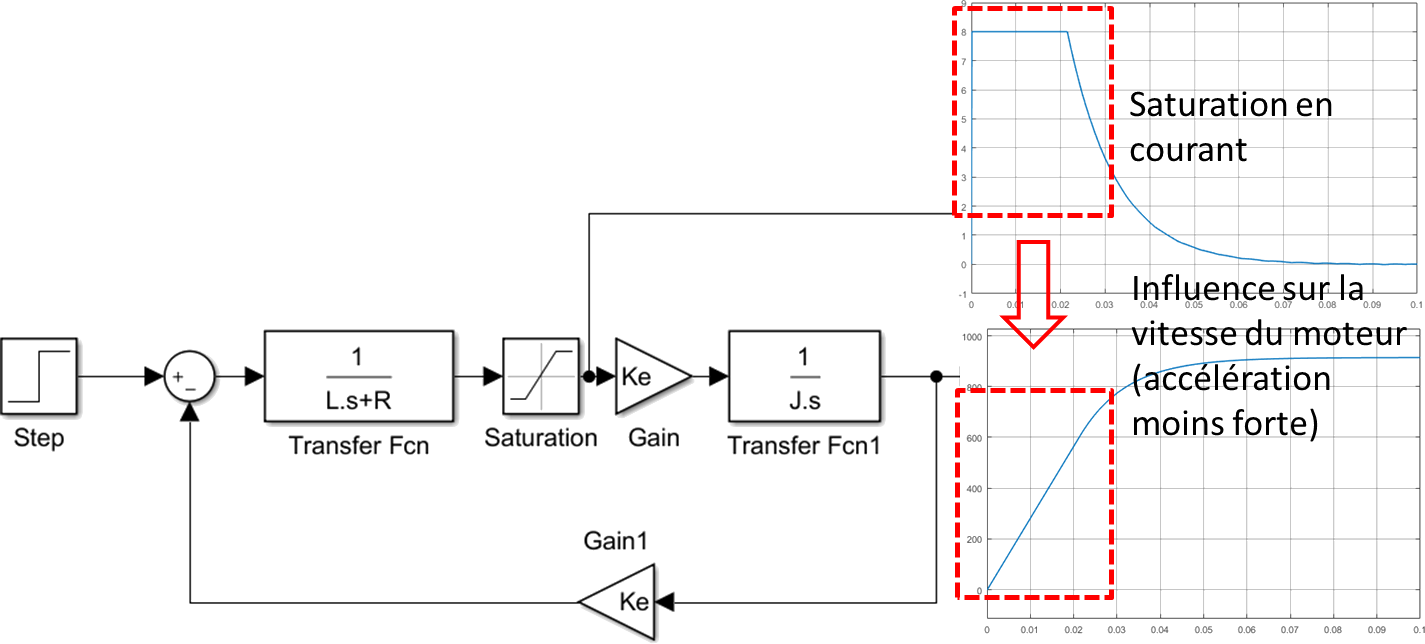
\includegraphics[width=\linewidth]{Modele_MCC_sat}
\end{marginfigure}
\begin{exemple}[title=Exemple] ~\\

%\begin{minipage}[c]{.48\linewidth}
Prenons par exemple le cas du moteur à continu du Maxpid dont la modélisation est (ou devrait être)  bien connue. Sollicitons le moteur par un échelon de tension et observons les signaux que nous ne regardons peut être pas toujours, par exemple le courant. 
Au démarrage du moteur, si on néglige la bobine et qu'on néglige l'existence d'une tension dans la boucle de retour, le courant initial est de l'ordre de $\dfrac{U}{R}\simeq \dfrac{48}{2}=\SI{24}{A}$. Pour certain système ce courant peut détériorer des composants. Afin de limiter le courant, des saturateurs permettant d'éviter de dépasser certaines intensités. 

La conséquence peut ici être un ralentissement du système. En effet, le courant << plafonnant >>, l'accélération n'est pas aussi forte qu'on l'attendrait. En conséquence, le système est moins rapide. 
%\end{minipage}
%\hfill
%\begin{minipage}[c]{.48\linewidth}

%\end{minipage}

\end{exemple}

\subsection{Seuil}

\begin{marginfigure}
\centering
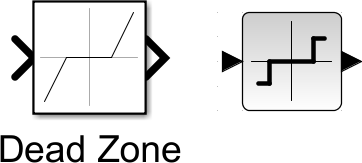
\includegraphics[width=3.5cm]{seuil}
Paramètres : valeur mini et valeur maxi
\end{marginfigure}

\begin{marginfigure}
\centering
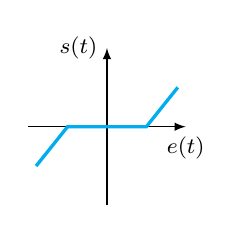
\begin{tikzpicture}
\draw [-latex] (0,-1) -- (0,1) node [left]{\footnotesize $s(t)$};
\draw [-latex] (-1,0) -- (1,0) node [below]{\footnotesize $e(t)$};
\draw [cyan,very thick] (-.9,-.5) -- (-.5,0) -- (.5,0) -- (.9,.5);
\end{tikzpicture}
\end{marginfigure}


Les seuils (ou bandes mortes -- dead band) permettent de modéliser un comportement non linéaire pour lequel la sortie reste nulle quand l'entrée varie dans un certain intervalle. 

Dans le cas d'une modélisation causale, on peut utiliser le seuil pour modéliser le frottement sec. En effet, dans le cas d'un système piloté par un moteur à courant continu, une petite tension ne suffit pas à actionner le système. Il faut vaincre les frottements secs. Le seuil permet de modéliser ce comportement.


\subsection{Hystérésis}

\begin{marginfigure}
\centering
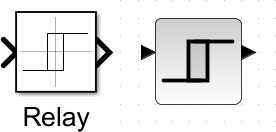
\includegraphics[width=3.5cm]{hysteresis}
Paramètres : switch on point, switch off point, output when on, output when off
\end{marginfigure}

\begin{marginfigure}
\centering
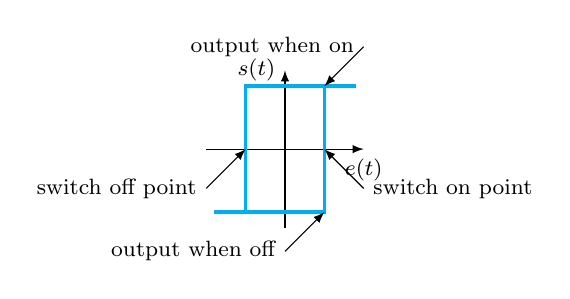
\begin{tikzpicture}
\draw [-latex] (0,-1) -- (0,1) node [left]{\footnotesize $s(t)$};
\draw [-latex] (-1,0) -- (1,0) node [below]{\footnotesize $e(t)$};
\draw [cyan,very thick] (-.9,-.8) -- (.5,-.8) -- (.5,.8) -- (.9,.8) -- (-.5,.8) -- (-.5,-.8);

\draw [latex-] (.5,0) --++(.5,-.5) node [right] {\footnotesize switch on point};
\draw [latex-] (-.5,0) --++(-.5,-.5) node [left] {\footnotesize switch off point};
\draw [latex-] (.5,.8) --++(.5,.5) node [left] {\footnotesize output when on};
\draw [latex-] (.5,-.8) --++(-.5,-.5) node [left] {\footnotesize output when off};
\end{tikzpicture}
\end{marginfigure}

Les hystérésis (Relay) permettent de modéliser un comportement non linéaire pour lequel la sortie est différente quand l'entrée croît ou lorsqu'elle décroit. 


\section{Modélisation des systèmes numériques}[Numérique]
On verra dans un chapitre ultérieur que les systèmes que nous manipulons sont souvent numériques. En effet, que ce soit sur le Maxpid, le Control'X, le D2C, la cheville NAO \textit{etc.} les grandeurs analogiques mesurées sont converties en grandeurs numériques grâce à un CAN (convertisseur analogique numérique). La fréquence d'échantillonnage ou la quantification du signal peuvent avoir un impact non négligeable sur les performances du système.

%De ce fait, un paramètre déterminant est la fréquence d'échantillonnage du système. Nous verrons son rôle dans un chapitre ultérieur.


%\begin{thebibliography}{2}
%   \bibitem[1]{ref1} Y. Crevits, {\it Éléments de modélisation multi-physique des systèmes industriels en vue de leur simulation numérique, Juin 2015.}
%   \bibitem[2]{ref2} Ph. Fichou, {\it La modélisation multiphysique, Technologie, Mars 2012.}
%   \bibitem[3]{ref3} Yvan Liebgott, {\it Modélisation et Simulation des Systemes Multi-Physiques avec MATLAB.}
%   \bibitem[4]{ref4} Frédéric Mazet, {\it Cours d'automatique de deuxième année, Lycée Dumont Durville, Toulon.}
%   \bibitem[5]{ref5} Patrick Beynet, {\it Sciences industrielles de l'ingénieur MP - PSI}
%, Éditions Ellipses.
%%      \bibitem[5]{ref5} Ivan Liebgott, {\it Modélisation et Simulation des systèmes Multi-Physiques avec MATLAB--Simulink.}
%
%\end{thebibliography}

